\newpage
\pagestyle{fancy}
\lhead{\textsc{Chapitre 2. Préparation du projet}}
\renewcommand{\headrulewidth}{0.5pt}
\renewcommand{\footrulewidth}{0.5pt}
\chapter{Préparation du projet}\setlength{\headheight}{28pt}
\label{ch2}
\thispagestyle{empty}
\minitoc
\newpage

Après avoir présenté le cadre général du projet, nous entamons la phase de préparation du projet
selon la méthodologie Scrum. Cette étape vise à identifier, analyser et modéliser les besoins du
système SAV, ainsi qu'à définir l'organisation du projet, l'environnement de travail et l'architecture
adoptée.

% ─────────────────────────────────────────────────────────────────────────────
\section{Capture des besoins}

\subsection{Spécification des besoins}

\subsubsection{Exigences fonctionnelles}

\begin{table}[H]
\centering
\caption{Exigences fonctionnelles}
\label{tab:ch2:exigences_fonctionnelles}
\begin{tabular}{|p{3.8cm}|p{10.7cm}|}
\hline
\textbf{Module} & \textbf{Description condensée} \\
\hline
Authentification & Connexion par e-mail ou téléphone, contrôle d'accès par rôle (RBAC), déconnexion sécurisée. \\
\hline
Utilisateurs & CRUD des comptes internes (administrateur, technicien) avec désactivation logique et restauration. \\
\hline
Clients & CRUD des fiches clients (société ou personne physique), ville tunisienne, accès portail client. \\
\hline
Équipements & Catalogue global (climatiseur, système de surpression) avec images multiples et image principale. \\
\hline
Affectation & Association équipement–client via \texttt{ClientEquipement} avec date d'achat, date d'installation et localisation. \\
\hline
Contrats & CRUD des contrats couvrant des installations \texttt{ClientEquipement} avec périodicité et statut calculé. \\
\hline
Planning préventif & Génération automatique des interventions préventives lors de la création d'un contrat. \\
\hline
Interventions & Cycle de vie complet (préventives et curatives), affectation technicien avec vérification de disponibilité. \\
\hline
Pannes & Déclaration par le client avec pièces jointes ; conversion en intervention curative par l'administrateur. \\
\hline
Facturation & Génération des factures pour interventions curatives hors contrat (TVA 19\,\%, TND) ; marquage payée. \\
\hline
Tableaux de bord & Dashboard global administrateur, dashboard personnel technicien, espace client différencié. \\
\hline
Historique & Consultation de l'historique des interventions filtrée selon le rôle de l'utilisateur connecté. \\
\hline
\end{tabular}
\end{table}

\subsubsection{Exigences non fonctionnelles}

\begin{table}[H]
\centering
\caption{Exigences non fonctionnelles}
\label{tab:ch2:exigences_nf}
\begin{tabular}{|p{3cm}|p{11.5cm}|}
\hline
\textbf{Exigence} & \textbf{Description} \\
\hline
Sécurité & Authentification obligatoire, contrôle d'accès RBAC, mots de passe chiffrés, session sans stockage en clair. \\
\hline
Performance & Temps de réponse rapide, listes paginées pour limiter le volume de données chargées. \\
\hline
Ergonomie & Interface en français, intuitive, responsive (desktop, tablette, mobile), thèmes clair et sombre. \\
\hline
Maintenabilité & TypeScript avec typage strict, architecture modulaire, composants réutilisables. \\
\hline
Disponibilité & Accessible depuis tout navigateur web moderne sans installation préalable. \\
\hline
Localisation & Monnaie TND, TVA 19\,\%, liste de villes tunisiennes intégrée. \\
\hline
Fiabilité & Validation des données côté client, messages d'erreur explicites. \\
\hline
\end{tabular}
\end{table}

% ─────────────────────────────────────────────────────────────────────────────
\section{Modélisation des besoins}

\subsection{Identification des acteurs}

Le système fait intervenir quatre acteurs ayant des rôles distincts :

\begin{table}[H]
\centering
\caption{Identification des acteurs}
\label{tab:ch2:acteurs}
\begin{tabular}{|p{3.2cm}|p{7.5cm}|}
\hline
\textbf{Acteur} & \textbf{Permissions principales} \\
\hline
\textbf{Administrateur}
  & Gère les utilisateurs, les clients, les équipements, les contrats, les interventions, les factures et le suivi global du système. \\
\hline
\textbf{Technicien}
  & Réalise les interventions, consulte son planning et son historique. \\
\hline
\textbf{Client}
  & Déclare les pannes, consulte ses factures, ses interventions et son historique. \\
\hline
\end{tabular}
\end{table}

\subsection{Identification des cas d'utilisation}

Les associations entre acteurs et cas d'utilisation sont représentées dans le diagramme global.
L'administrateur hérite des fonctionnalités du technicien, tandis que le client dispose d'un accès
limité aux fonctions de déclaration et de consultation.

\subsection{Diagramme de cas d'utilisation global}

\begin{figure}[H]
\centering
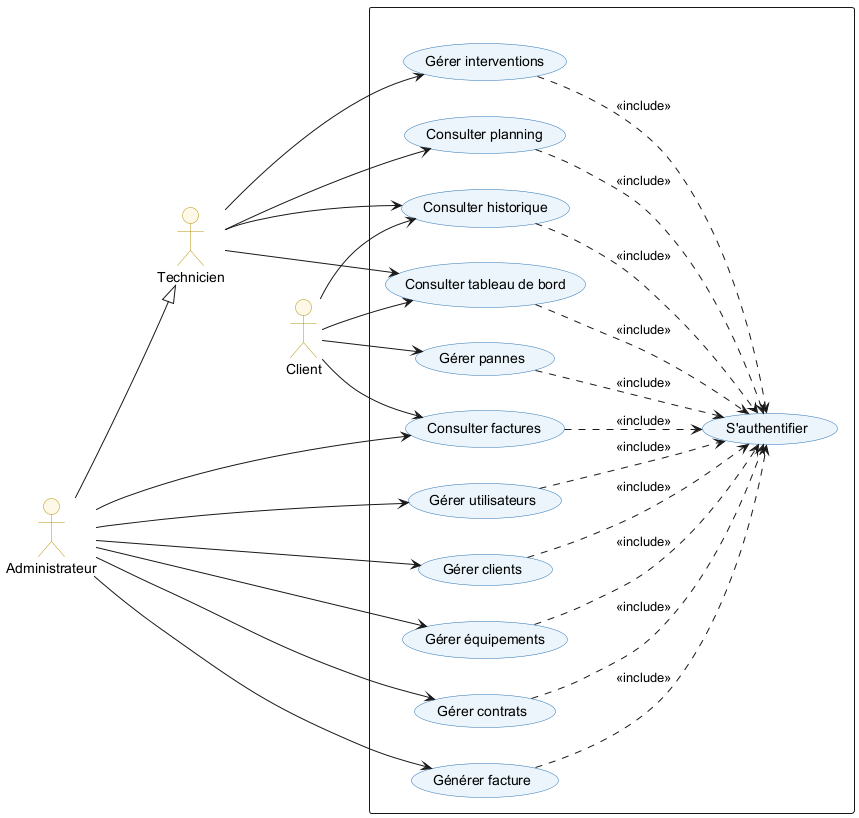
\includegraphics[width=0.7\textwidth]{Figures/Chapitre1/globaluasecase.png}
\caption{Diagramme de cas d'utilisation global}
\label{fig:ch2:usecase_global}
\end{figure}

% ─────────────────────────────────────────────────────────────────────────────
\section{Diagramme de classes global}

Le diagramme de classes global représente la structure générale du système ainsi que les relations
entre les onze entités principales.

\begin{figure}[H]
\centering
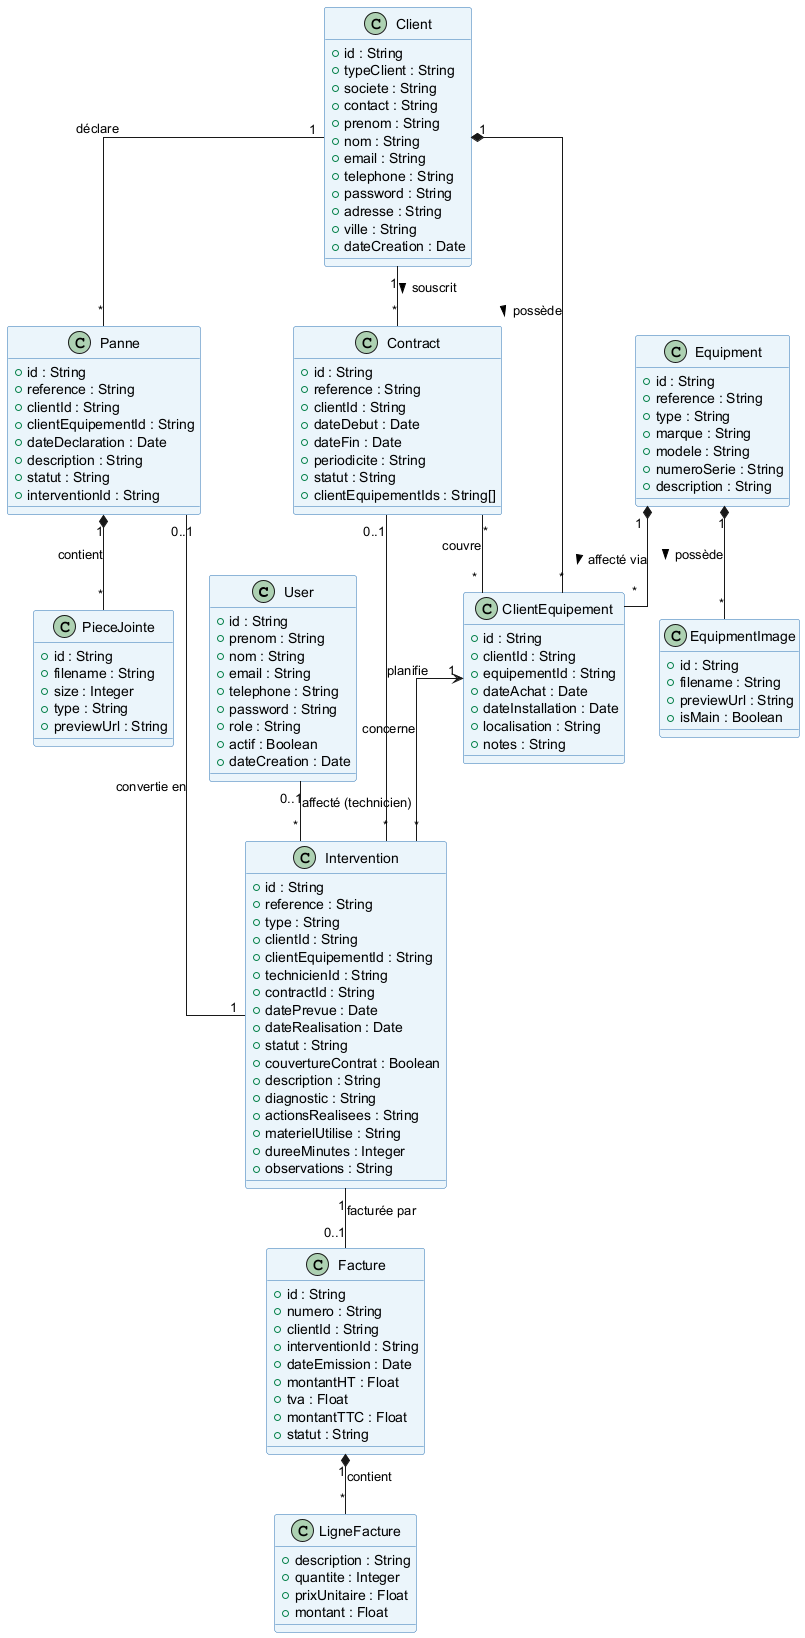
\includegraphics[width=0.8\textwidth]{Figures/Chapitre1/globaldiagramclass.png}
\caption{Diagramme de classes global}
\label{fig:ch2:class_global}
\end{figure}

\textbf{Dictionnaire de données :}

\begin{longtable}{|p{3.2cm}|p{11.3cm}|}
\caption{Dictionnaire de données}
\label{tab:ch2:dictionnaire} \\
\hline
\textbf{Entité} & \textbf{Description} \\
\hline
\endfirsthead
\caption*{Dictionnaire de données (suite)} \\
\hline
\textbf{Entité} & \textbf{Description} \\
\hline
\endhead
\hline
\endfoot
\hline
\endlastfoot
\texttt{User}
  & Utilisateur interne (administrateur ou technicien).
    Attributs : prenom, nom, email, role (\texttt{admin}/\texttt{technician}), actif. \\
\hline
\texttt{Client}
  & Client métier (société ou personne physique).
    Attributs : typeClient, societe, prenom, nom, email, adresse, ville. \\
\hline
\texttt{Equipment}
  & Équipement du catalogue global, indépendant de tout client.
    Attributs : reference, type (\texttt{CLIMATISEUR}/\texttt{SYSTEME\_SURPRESSION}), marque, modele, numeroSerie. \\
\hline
\texttt{EquipmentImage}
  & Image associée à un équipement.
    Attribut notable : isMain (désigne l'image principale). \\
\hline
\texttt{ClientEquipement}
  & Table de jonction \texttt{Client}–\texttt{Equipment} matérialisant une installation.
    Attributs : dateAchat, dateInstallation, localisation (optionnel). \\
\hline
\texttt{Contract}
  & Contrat de maintenance couvrant des installations \texttt{ClientEquipement}.
    Attributs : reference, dateDebut, dateFin, periodicite, statut (\texttt{ACTIF}/\texttt{BIENTOT\_EXPIRE}/\texttt{EXPIRE}). \\
\hline
\texttt{Intervention}
  & Intervention préventive ou curative, sans champ de priorité.
    Attributs : type (\texttt{PREVENTIVE}/\texttt{CURATIVE}), datePrevue, statut (\texttt{PLANIFIEE}/\texttt{EN\_COURS}/\texttt{REALISEE}/\texttt{ANNULEE}), couvertureContrat. \\
\hline
\texttt{Panne}
  & Déclaration de panne par un client, sans champ de priorité.
    Attributs : dateDeclaration, description, statut (\texttt{EN\_ATTENTE}/\texttt{PRISE\_EN\_CHARGE}/\texttt{CONVERTIE}/\texttt{ANNULEE}). \\
\hline
\texttt{PieceJointe}
  & Pièce jointe associée à une panne.
    Attributs : filename, size, type (image, PDF ou audio). \\
\hline
\texttt{Facture}
  & Facture pour une intervention curative réalisée hors contrat.
    Attributs : numero, dateEmission, montantHT, tva (19\,\%), montantTTC, statut (\texttt{PAYEE}/\texttt{IMPAYEE}/\texttt{EN\_ATTENTE}). \\
\hline
\texttt{LigneFacture}
  & Ligne de détail d'une facture.
    Attributs : description, quantite, prixUnitaire, montant. \\
\hline
\end{longtable}

% ─────────────────────────────────────────────────────────────────────────────
\section{Pilotage du projet avec Scrum}

\subsection{Équipe et rôles}

Le projet est organisé selon la méthodologie Scrum. Les rôles principaux sont :

\begin{table}[H]
\centering
\caption{Équipe et rôles Scrum}
\label{tab:ch2:roles}
\begin{tabular}{|p{4.5cm}|p{10cm}|}
\hline
\textbf{Rôle} & \textbf{Description} \\
\hline
\textbf{Product Owner}
  & Définit les besoins fonctionnels du projet et priorise le backlog \\
\hline
\textbf{Scrum Master}
  & Assure le suivi de la méthodologie Scrum et facilite les cérémonies \\
\hline
\textbf{Équipe de développement}
  & Réalise l'analyse, la conception et le développement des fonctionnalités \\
\hline
\end{tabular}
\end{table}

\subsection{Le Backlog du produit}

Le backlog complet comporte 28 user stories. Le tableau suivant présente les user stories représentatives couvrant les principaux modules du système.

\begin{longtable}{|p{1.2cm}|p{7.5cm}|p{2.3cm}|p{1.5cm}|p{1.2cm}|}
\caption{Product Backlog --- sélection représentative (28 user stories au total)}
\label{tab:ch2:backlog} \\
\hline
\textbf{ID} & \textbf{User Story} & \textbf{Acteur} & \textbf{Priorité} & \textbf{Sprint} \\
\hline
\endfirsthead
\caption*{Product Backlog (suite)} \\
\hline
\textbf{ID} & \textbf{User Story} & \textbf{Acteur} & \textbf{Priorité} & \textbf{Sprint} \\
\hline
\endhead
\hline
\endfoot
\hline
\endlastfoot
US-01 & En tant qu'utilisateur, je veux me connecter avec mon e-mail ou mon numéro de téléphone et mon mot de passe. & Tout utilisateur & Haute & S1 \\
\hline
US-04 & Le système restreint automatiquement l'accès aux pages selon le rôle de l'utilisateur. & Système (auto) & Haute & S1 \\
\hline
US-08 & En tant qu'administrateur, je veux affecter un équipement du catalogue à un client via \texttt{ClientEquipement}. & Administrateur & Haute & S1 \\
\hline
US-09 & En tant qu'administrateur, je veux créer un contrat couvrant des installations \texttt{ClientEquipement}. & Administrateur & Haute & S1 \\
\hline
US-11 & En tant qu'administrateur, je veux affecter un technicien disponible à une intervention. & Administrateur & Haute & S2 \\
\hline
US-16 & En tant que client, je veux déclarer une panne avec pièces jointes. & Client & Haute & S2 \\
\hline
US-19 & En tant qu'administrateur, je veux générer une facture pour une intervention curative réalisée hors contrat (TVA 19\,\%, TND). & Administrateur & Haute & S3 \\
\hline
US-25 & En tant qu'administrateur, je veux consulter un tableau de bord global avec KPIs et graphiques. & Administrateur & Haute & S3 \\
\hline
\end{longtable}

\subsection{Planification des sprints}

\begin{longtable}{|p{1.7cm}|p{3.2cm}|p{5.8cm}|p{4cm}|}
\caption{Planification des sprints}
\label{tab:ch2:sprints} \\
\hline
\textbf{Sprint} & \textbf{Objectif} & \textbf{Fonctionnalités couvertes} & \textbf{Entités concernées} \\
\hline
\endfirsthead
\hline
\textbf{Sprint} & \textbf{Objectif} & \textbf{Fonctionnalités couvertes} & \textbf{Entités concernées} \\
\hline
\endhead
\hline
\endfoot
\hline
\endlastfoot
\textbf{Sprint 1}
  & Authentification et référentiel métier
  & Connexion (email ou téléphone), contrôle d'accès RBAC ;
    CRUD utilisateurs (soft-delete), clients et équipements ;
    affectation \texttt{ClientEquipement} ; contrats et planning préventif automatique.
  & \texttt{User}, \texttt{Client}, \texttt{Equipment},
    \texttt{EquipmentImage}, \texttt{ClientEquipement},
    \texttt{Contract} \\
\hline
\textbf{Sprint 2}
  & Gestion des interventions et des pannes
  & Affectation technicien (vérification disponibilité) ;
    démarrage et clôture interventions ;
    déclaration panne avec pièces jointes ;
    conversion panne $\rightarrow$ curative ; vérification couverture contractuelle.
  & \texttt{Intervention}, \texttt{Panne}, \texttt{PieceJointe},
    \texttt{Contract}, \texttt{ClientEquipement} \\
\hline
\textbf{Sprint 3}
  & Facturation, historique et tableaux de bord
  & Génération factures (curative + hors contrat, TVA 19\,\%) ;
    marquage payée ; historique par rôle ;
    dashboards administrateur, technicien et client.
  & \texttt{Facture}, \texttt{LigneFacture}, \texttt{Intervention},
    \texttt{Client}, \texttt{User} \\
\hline
\end{longtable}

% ─────────────────────────────────────────────────────────────────────────────
\section{Environnement de travail}

\subsection{Environnement matériel}

Le développement de l'application a été réalisé avec les équipements suivants :

\begin{table}[H]
\centering
\caption{Environnement matériel}
\label{tab:ch2:materiel}
\begin{tabular}{|p{4cm}|p{10cm}|}
\hline
\textbf{Élément} & \textbf{Caractéristiques} \\
\hline
Machine      & PC Portable \\
\hline
Processeur   & Intel Core i5 \\
\hline
Mémoire RAM  & 8 Go \\
\hline
Stockage     & SSD 512 Go \\
\hline
\end{tabular}
\end{table}

\subsection{Environnement logiciel}

\begin{table}[H]
\centering
\caption{Environnement logiciel}
\label{tab:ch2:logiciel}
\begin{tabular}{|p{4cm}|p{10cm}|}
\hline
\textbf{Outil} & \textbf{Description} \\
\hline
Visual Studio Code & Environnement de développement intégré \\
\hline
Next.js            & Framework Frontend (App Router) \\
\hline
React              & Bibliothèque JavaScript \\
\hline
TypeScript         & Typage statique strict \\
\hline
Tailwind CSS       & Framework CSS utilitaire \\
\hline
Prisma             & ORM pour la base de données \\
\hline
MySQL              & Système de gestion de base de données \\
\hline
\end{tabular}
\end{table}

% ─────────────────────────────────────────────────────────────────────────────
\section{Architecture de l'application}

L'application est construite sur une architecture web en trois couches qui sépare clairement le
frontend, la logique métier et la base de données.

\textbf{Couche présentation (Frontend)} Le frontend de l'application est développé en utilisant
Next.js et React. Cette combinaison permet de créer une interface utilisateur à la fois moderne
et dynamique. Les composants React assurent une séparation claire des responsabilités d'affichage.

\textbf{Couche logique métier (Backend / API)} La couche backend expose des routes API RESTful
implémentées sous forme de contrôleurs. Chaque contrôleur gère la validation des données,
l'exécution de la logique métier et les appels vers la base de données.

\textbf{Couche d'accès aux données (Prisma / MySQL)} L'accès à la base de données est géré
via Prisma ORM. Cette couche exécute les requêtes vers la base de données MySQL et garantit
l'intégrité des données via la gestion des transactions (COMMIT/ROLLBACK).

\begin{figure}[H]
\centering
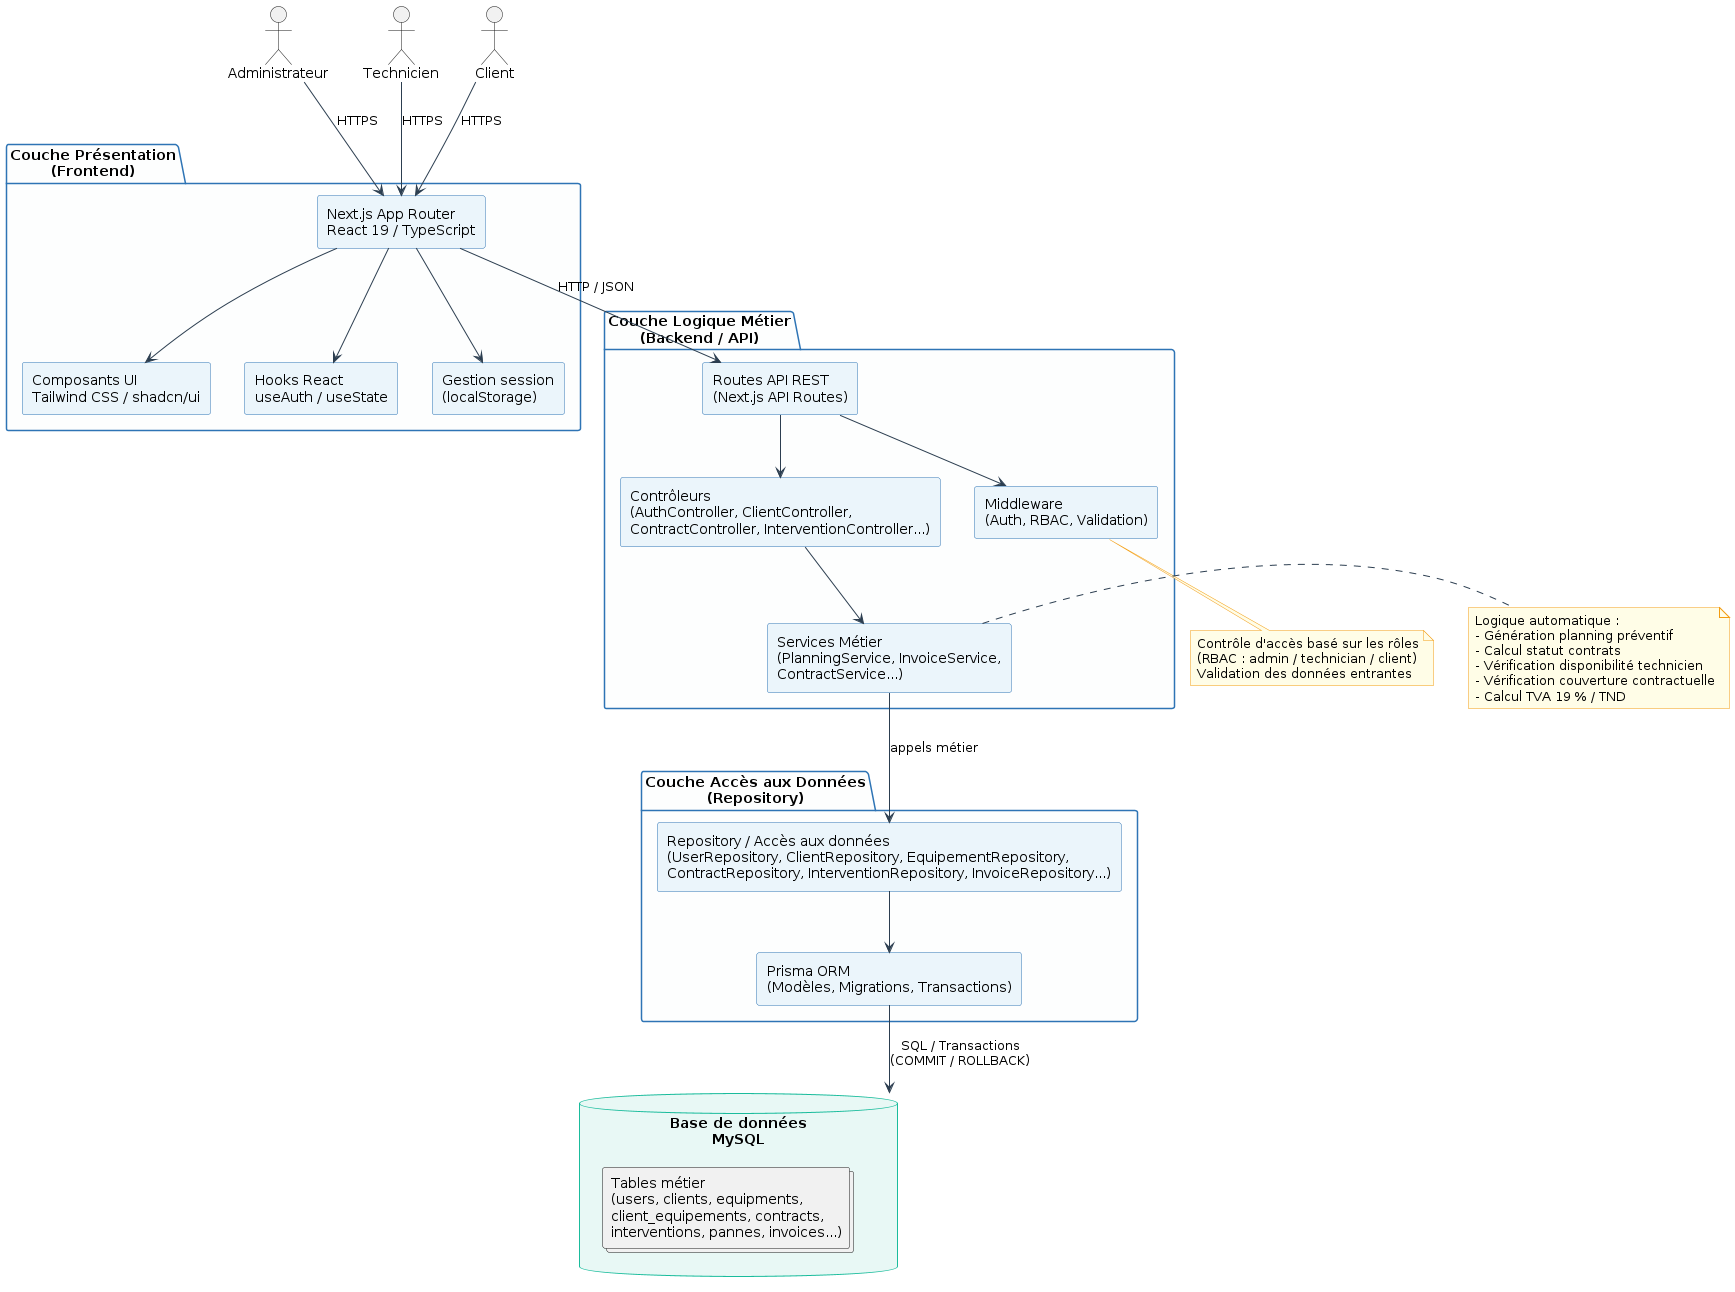
\includegraphics[width=0.8\textwidth]{Figures/Chapitre2/architecture.png}
\caption{Architecture de l'application}
\label{fig:ch2:architecture}
\end{figure}

% ─────────────────────────────────────────────────────────────────────────────
\section*{Conclusion}

Dans ce chapitre, nous avons établi les exigences fonctionnelles et non fonctionnelles de
l'application en précisant leurs règles métier. Nous avons identifié trois acteurs
(Administrateur, Technicien et Client) et représenté leurs interactions à travers 28
User Stories réparties sur 3 sprints. Le schéma de classes global présente les 11 entités du
modèle, incluant l'entité intermédiaire \texttt{ClientEquipement} qui associe les clients aux
équipements du catalogue. Le prochain chapitre traitera du Sprint 1 --- Authentification et
référentiel métier.
